\section{Experiments}

We evaluate whether selective perception improves event recall and latency under fixed budgets.

\paragraph{Baselines.}
We compare against random scheduling, uniform round-robin scheduling, motion top-$k$, anomaly-score top-$k$, CLIP prompt top-$k$, and dense VLM inspection. Dense inspection is an upper-cost reference rather than a deployable baseline.

\paragraph{Main results.}
Table~\ref{tab:main-results} reports results at a fixed per-timestep VLM-call budget. \method{} improves event recall by 10.8 percentage points over CLIP prompt top-$k$ and 15.0 points over anomaly top-$k$. It also reduces mean time-to-detect and false alarms. Dense VLM inspection has the highest recall, but costs 7420 GPU-seconds per hour, compared with 1088 for \method.

\begin{table}[t]
\centering
\caption{Main results under a fixed VLM-call budget. Numbers are reported at the episode level and aggregated over benchmark tracks.}
\label{tab:main-results}
\begin{tabular}{lrrrrr}
\toprule
Method & Recall@B $\uparrow$ & TTD (s) $\downarrow$ & FA/h $\downarrow$ & GPU-s/h $\downarrow$ & VLM calls/event $\downarrow$ \\
\midrule
Random scheduler & 41.2 & 72.8 & 7.84 & 1050 & 38.5 \\
Uniform round-robin & 46.8 & 65.1 & 6.97 & 1050 & 38.5 \\
Motion top-k & 57.4 & 49.7 & 9.36 & 1050 & 38.5 \\
Anomaly-score top-k & 64.1 & 43.9 & 8.12 & 1050 & 38.5 \\
CLIP prompt top-k & 68.3 & 39.4 & 6.44 & 1050 & 38.5 \\
Dense VLM every stream & 86.1 & 21.7 & 4.91 & 7420 & 271.6 \\
\textbf{TriageVLM} & 79.1 & 28.6 & 4.38 & 1088 & 39.9 \\
\bottomrule
\end{tabular}

\end{table}

\begin{figure}[t]
\centering
\resizebox{0.92\linewidth}{!}{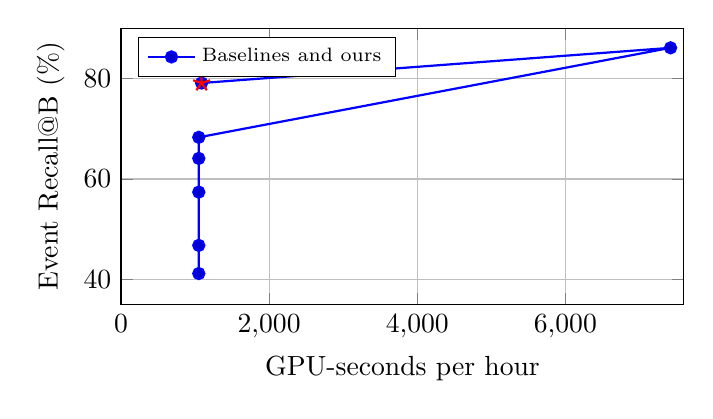
\begin{tikzpicture}
\begin{axis}[
  width=0.72\linewidth,
  height=0.42\linewidth,
  xlabel={GPU-seconds per hour},
  ylabel={Event Recall@B (\%)},
  xmin=0,
  xmax=7600,
  ymin=35,
  ymax=90,
  grid=both,
  legend style={at={(0.03,0.97)},anchor=north west,font=\scriptsize},
]
\addplot+[mark=*, thick] coordinates {(1050,41.199999999999996) (1050,46.800000000000004) (1050,57.4) (1050,64.1) (1050,68.30000000000001) (7420,86.1) (1088,79.10000000000001)};
\addlegendentry{Baselines and ours}
\addplot+[only marks, mark=star, mark size=3.2pt, thick] coordinates {(1088,79.10000000000001)};
\end{axis}
\end{tikzpicture}
}
\caption{Cost-performance frontier. \method{} sits near dense VLM recall while operating close to the sparse scheduler compute regime.}
\label{fig:frontier}
\end{figure}

\paragraph{Detection latency.}
Figure~\ref{fig:ttd-cdf} shows time-to-detect distributions for detected events. \method{} shifts detections earlier, which is critical in monitoring even when final recall is similar.

\begin{figure}[t]
\centering
\resizebox{0.92\linewidth}{!}{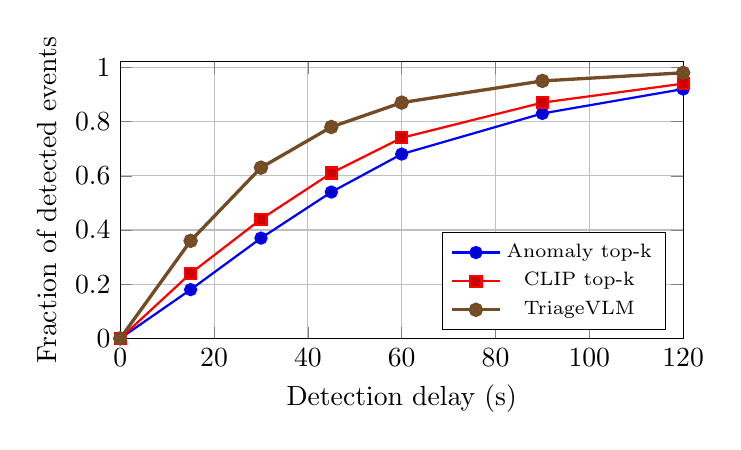
\begin{tikzpicture}
\begin{axis}[
  width=0.72\linewidth,
  height=0.42\linewidth,
  xlabel={Detection delay (s)},
  ylabel={Fraction of detected events},
  xmin=0, xmax=120, ymin=0, ymax=1.02,
  grid=both,
  legend style={at={(0.97,0.03)},anchor=south east,font=\scriptsize},
]
\addplot+[thick] coordinates {(0,0.0) (15,0.18) (30,0.37) (45,0.54) (60,0.68) (90,0.83) (120,0.92)};
\addlegendentry{Anomaly top-k}
\addplot+[thick] coordinates {(0,0.0) (15,0.24) (30,0.44) (45,0.61) (60,0.74) (90,0.87) (120,0.94)};
\addlegendentry{CLIP top-k}
\addplot+[very thick] coordinates {(0,0.0) (15,0.36) (30,0.63) (45,0.78) (60,0.87) (90,0.95) (120,0.98)};
\addlegendentry{TriageVLM}
\end{axis}
\end{tikzpicture}
}
\caption{Cumulative distribution of detection delays. A larger fraction of \method{} detections occur within the first 30 seconds after event onset.}
\label{fig:ttd-cdf}
\end{figure}

\paragraph{Ablations.}
Table~\ref{tab:ablation} shows that each component contributes. Removing event memory hurts persistent event recovery; removing CLIP prompt similarity weakens semantic incident routing; removing the anomaly prior reduces rare-event sensitivity; and removing cooldown increases false alarms.

\begin{table}[t]
\centering
\caption{Ablation at the same VLM-call budget.}
\label{tab:ablation}
\begin{tabular}{lrrrr}
\toprule
Variant & Recall@B $\uparrow$ & TTD (s) $\downarrow$ & FA/h $\downarrow$ & Calls/event $\downarrow$ \\
\midrule
TriageVLM & 79.1 & 28.6 & 4.38 & 39.9 \\
w/o event memory & 74.2 & 35.1 & 5.62 & 39.9 \\
w/o uncertainty bonus & 75.7 & 33.8 & 4.91 & 39.9 \\
w/o CLIP prompt score & 72.1 & 37.5 & 5.14 & 39.9 \\
w/o anomaly prior & 70.4 & 40.8 & 4.72 & 39.9 \\
greedy no cooldown & 73.1 & 34.9 & 8.07 & 39.9 \\
\bottomrule
\end{tabular}

\end{table}
